\section{Diversity im Reinforcement Learning}
\label{sec:diversity}
% Ziel
In diesem Kapitel beschäftigen wir uns damit, wie das Konzept von Diversity im Bereich des Reinforcement Learning (RL) Anwendung finden kann. Ziel ist, dass ein RL Agent in einer unüberwachten Phase zunächst Fähigkeiten erlernt, welche das Bewältigen von Aufgaben in der darauf folgenden, überwachten Phase erleichtern sollen.

Dieses Kapitel stützt sich zu einem Großteil auf die wissenschaftliche Arbeit \textit{Diversity is all you need: Learning skills without a reward function}\cite{diversity_eysenbach}. Falls nicht anders angegeben, wurden die Informationen hieraus entnommen.

% Grundlegende Begriffe
\subsection{Klärung wichtiger Begriffe aus der Informationstheorie}
\label{sec:informationtheory}
Im Folgenden werden Begriffe aus der Informationstheorie verwendet, welche es zunächst zu klären gilt. Wir betrachten \textit{Entropie} und \textit{Transinformation} nach \cite{elements_cover} und \cite{information_werner}.

\smallspace

Die \textit{Entropie} beschreibt in der Informationstheorie den mittleren Informationsgehalt bzw. die Ungewissheit einer Quelle. Ist beispielsweise bei einer Ereignismenge jedes Ereignis gleich wahrscheinlich, so ist die Ungewissheit maximal \cite{information_werner}.

Nach \cite{elements_cover} besitzt eine diskrete Zufallsvariable $ X $ mit dem Zeichenvorrat $ \mathcal{X} $ und der Wahrscheinlichkeitsfunktion $ p(x) $ die \textit{Entropie}
\begin{equation*}
    H(X) = -\sum_{x \in \mathcal{X}} p(x) \cdot log\ p(x) \label{eq:entropy}
\end{equation*}

Diese lässt sich nach \cite{elements_cover} auch über den Erwartungswert $ E $ berechnen unter Verwendung von
\begin{equation*}
    H(X) = E_p\ log\ \frac{1}{p(X)} \label{eq:entropy_1}
\end{equation*}
, woraus unter Anwendung der Rechenregeln für Logarithmus und Erwartungswert trivial
\begin{equation}
    H(X) = - E_p\ log\ p(X) \label{eq:entropy_2}
\end{equation}
folgt.

Desweiteren ist die Formel für die \textit{bedingte Entropie} nach \cite{elements_cover} gegeben durch
\begin{equation}
    H(Y|X) = - E_{p(x,y)}\ log\ p(Y|X) \label{eq:condit_entropy}
\end{equation}

\smallspace

Die \textit{Transinformation} beschreibt die Menge an Information, die eine Zufallsvariable über eine andere enthält bzw. die Reduktion der Ungewissheit aufgrund des Wissens um die jeweils andere Zufallsvariable \cite{elements_cover}.

Mathematisch wichtig für uns ist lediglich der Zusammenhang zwischen \textit{Transinformation} und \textit{Entropie}, welcher nach \cite{elements_cover} gegeben ist durch
\begin{equation}
    I(X;Y) = H(X) - H(X|Y) = H(Y) - H(Y|X) \label{eq:trans_ent}
\end{equation}

% Erklärung des Algorithmus
\subsection{Funktionsweise}
\label{sec:howitworks}
\begin{figure}
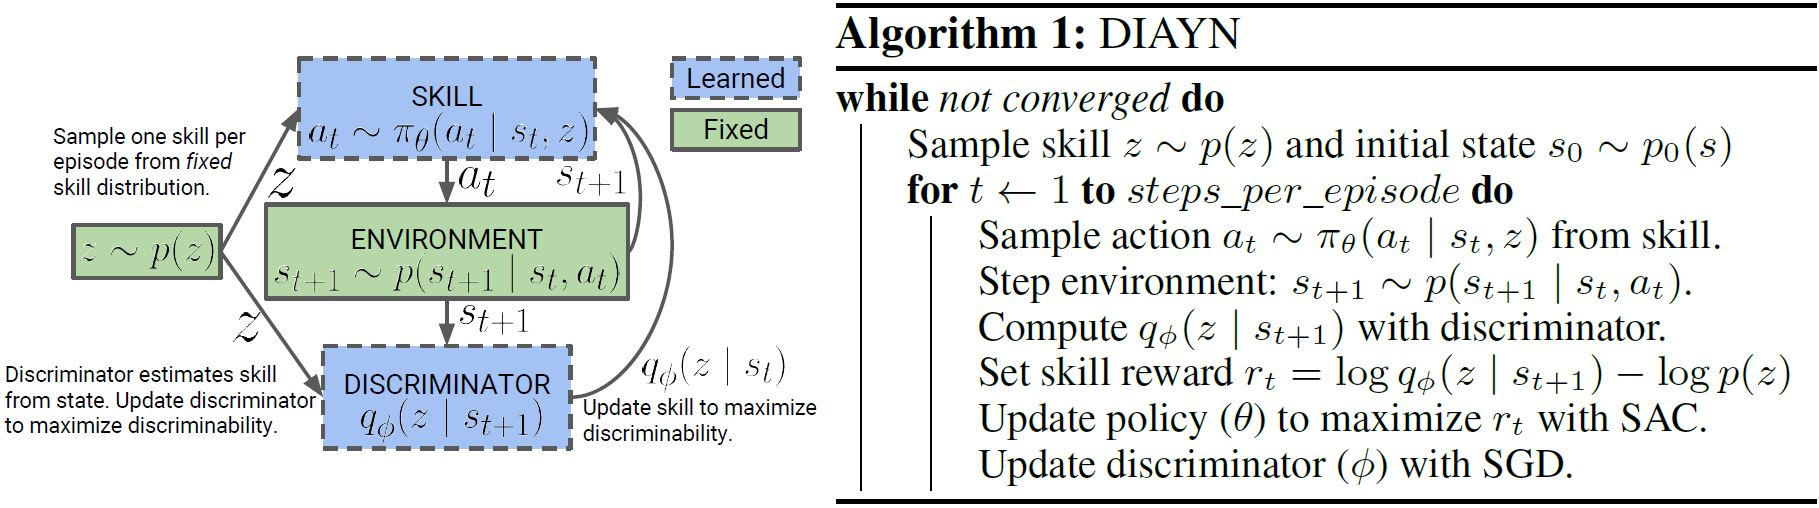
\includegraphics[width=\textwidth, keepaspectratio=true]{images/algorithm_diayn.JPG}
\caption{``Diversity is all you need'' Algorithmus} \label{img:diayn}
\source{\cite{diversity_eysenbach}}
\end{figure}
Das selbstständige Erlernen von brauchbaren Fähigkeiten, so wie in \cite{diversity_eysenbach} beschrieben, baut auf drei Grundideen auf.

\smallspace

Unterschiedliche Fähigkeiten sollten andere Zustände besuchen, sodass ihre Unterscheidbarkeit gewährleistet ist.

%TODO "Paper"
Um besagte Fähigkeiten zu unterscheiden, werden nicht die Aktionen, sondern die Zustände betrachtet. Das liegt daran, dass Aktionen, welche die Umgebung nicht beeinflussen, für einen Beobachter nicht erkennbar sind. Das Paper verdeutlicht dies mit einem treffenden Beispiel. Für einen außenstehenden Betrachter ist nicht ersichtlich, wie fest ein Roboterarm eine Tasse in der Hand hält, falls sich diese nicht bewegt.

Schließlich soll erreicht werden, dass die Fähigkeiten so vielfältig (\textit{diverse}) wie möglich sind. Die Idee ist, dass unterscheidbare Fähigkeiten mit einer hohen Entropie einen Zustandsraum abdecken, welcher sich weit entfernt von anderen Fähigkeiten befindet.

\smallspace

Um diese Punkte zu realisieren, definieren wir zunächst die Zufallsvariablen $ S $ und $ A $ für Zustände und Aktionen. Sei nun $ Z \sim p(z) $ eine latente Variable, unter deren Bedingung die Strategie definiert wird. Bei fixem $ Z $ sprechen wir hier von einer "Fähigkeit". Entropie sowie Transinformation werden zur Basis $ e $ berechnet.

Nun soll die Transinformation zwischen Fähigkeiten und Zuständen, $ I(S;Z) $, maximiert werden um sicherzustellen, dass die Fähigkeit die vom Agent durchlaufenen Zustände vorgibt. Anders gesagt wird sichergestellt, dass aus den besuchten Zuständen auf die Fähigkeit geschlossen werden kann.

Außerdem minimieren wir die Transinformation zwischen Fähigkeit und Aktionen bei gegebenen Zustand, $ I(A; Z | S) $. So wird garantiert, dass nicht Aktionen, sondern Zustände für die Unterscheidung von Fähigkeiten verwendet werden.

% unklar
Maximiert wird auch die Entropie $ H(A|S) $.

\smallspace

Insgesamt maximieren wir nach \cite{diversity_eysenbach} also
\begin{align}
    \mathcal{F}(\theta) &\stackrel{\triangle}{=} I(S;Z) + H(A|S) - I(A;Z|S) \label{eq:objective_1}\\
    & = (H(Z) - H(Z|S)) + H(A|S) - (H(A|S) - H(A|S,Z)) \nonumber\\
    & = H(Z) - H(Z|S) + H(A|S,Z) \label{eq:objective_intuitive}
\end{align}
Der Term wurde unter Verwendung von \eqref{eq:trans_ent} umgeformt.

Da sich $ p(z|S) $ nicht genau berechnen lässt, wird das Folgende mit einem discriminator $ q_\phi $ approximiert. Mit der Jensenschen Ungleichung haben wir laut \cite{diversity_eysenbach} eine untere Schranke $ \mathcal{G}(\theta) $ für $ \mathcal{F}(\theta, \phi) $:
\begin{align}
    \mathcal{F}(\theta) & = H(A|S,Z) - H(Z|S) + H(Z) \nonumber\\
    & = H(A|S,Z) + E_{z \sim p(z), s \sim \pi(z)}(log\ p(z | s)) - E_{z \sim p(z)}(log\ p(z)) \label{eq:objective_2}\\
    & \ge H(A|S,Z) + E_{z \sim p(z), s \sim \pi(z)}(log\ q_\phi(z | s) - log\ p(z)) \stackrel{\triangle}{=} \mathcal{G}(\theta, \phi) \nonumber
\end{align}
In \eqref{eq:objective_2} wurden die Entropien nach \eqref{eq:entropy_2} und \eqref{eq:condit_entropy} umgeformt.

\smallspace


% Beispiele
\subsection{Beispiele}
\label{sec:examplesdiversity}